% motivation
\subsection{Motivation: A sample experiment}
\label{motivation:example}
To demonstrate how a simulation experiment can be described simply and effectively, we make use of a rather simple, though famous, model that may yet display rich and variable behaviors. The simulation example is taken from \citep{Waltemath:2010}. 

The \emph{repressilator} is a synthetic oscillating network of transcription regulators in Escherichia coli \citep{Elowitz:2000}.
 The network is composed of the three repressor genes Lactose Operon Repressor (lacI), Tetracycline Repressor (tetR) and Repressor CI (cI), which code for proteins binding to the promoter of the other, blocking their transcription. The three inhibitions toghether in tandem, form a cyclic negative-feedback loop. 
To describe the interactions of the molecular species involved in the network, the authors built a simple mathematical model of coupled first-order differential equations. All six molecular species included in the network (three mRNAs, three repressor proteins) participated in creation (transcription/translation) and degradation processes. The model was used to determine the influence of the various parameters on the dynamic behavior of the system. In particular, parameter values were sought which induce stable oscillations in the concentrations of the system components. Oscillations in the levels of the three repressor proteins are obtained by numerical integration. 

\subsubsection{A simple time-course simulation}
\label{sec:intro1}
The first experiment we intend to run on the model is the simulation that will lead to the oscillation shown in Figure 1c of the reference publication \citep{Elowitz:2000}. The according simulation experiment can be described as:

\begin{enumerate}
	\item{Import the model identified by the Unified Resource Identifier \citep{Berners-Lee:2005} \url{urn:miriam:biomodels.db:BIOMD0000000012}.}

%  or \url{http://models.cellml.org/exposure/bee9fb9df261ba69b51897f2e49b1691/elowitz\_leibler\_2000.cellml.index.html} (for the CellML model)

	\item{Select a deterministic method.}
	\item{Run a uniform time course simulation for 1000~min with an output interval of 1~min.}
	\item{Plot the amount of \code{lacI}, \code{tetR} and \code{cI} against time in a 2D Plot.}
\end{enumerate}

Following those steps and performing the simulation in the simulation tool COPASI \citep{Hoops:2006} let to the result shown in \fig{simEx1}. 

\begin{figure}
\centering
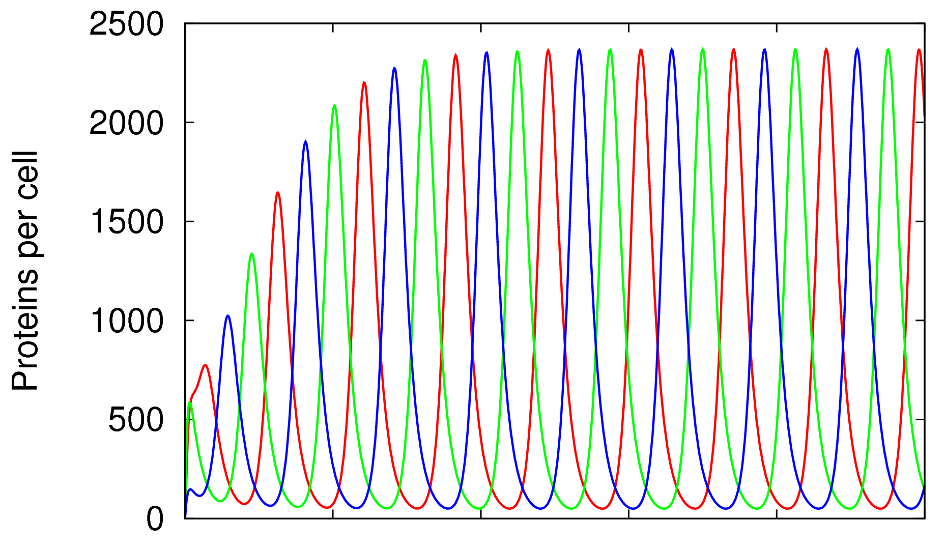
\includegraphics[width=0.6\textwidth]{images/simEx1.png}
\caption{Time-course simulation of the repressilator model, imported from BioModels Database and simulated in COPASI. The number of repressor proteins lacI, tetR and cI is shown. (taken from \citep{Waltemath:2010})}
\label{fig:simEx1}
\end{figure}

\subsubsection{Applying pre-processing}
The fine-tuning of the model can be shown by adjusting parameters before simulation. When changing the initial values of the parameters \emph{protein copies per promoter} and \emph{leakiness in protein copies per promoter} the system's behavior switches from sustained oscillation to asymptotic steady-state. The adjustments leading to that behavior may be described as: 
\begin{enumerate}
\item{Import the model as above.}
\item{Change the value of the parameter \code{tps$\_$repr} from “0.0005” to “1.3e-05”. }
\item{Change the value of the parameter \code{tps$\_$active} from “0.5 “ to “ 0.013“.}
\item{Select a deterministic method.}
\item{Run a uniform time course for the duration of 1000~min with an output interval of 1~min.}
\item Plot the amount of lacI, tetR and cI against time in a 2D Plot.
\end{enumerate}
\fig{simEx3} shows the result of the simulation.
%
\begin{figure}
\centering
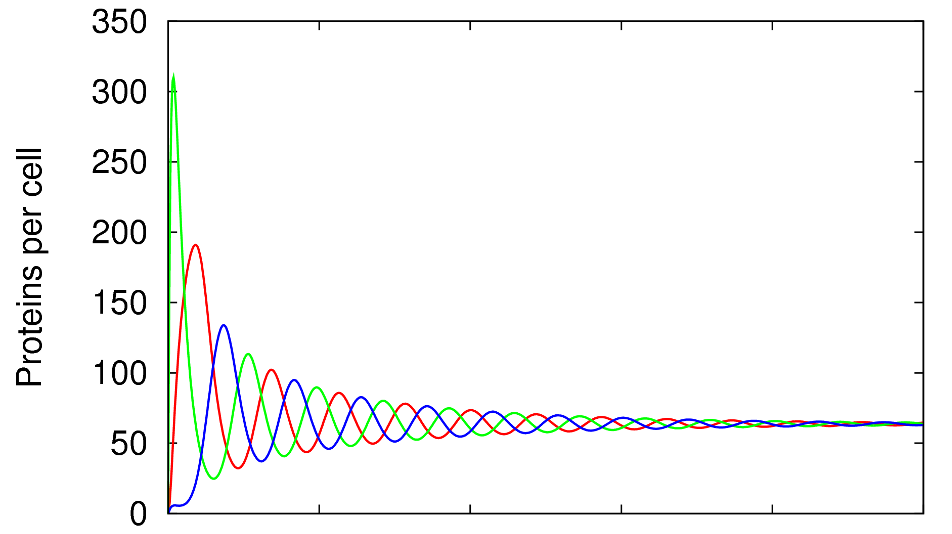
\includegraphics[width=0.7\textwidth]{images/simEx3.png}
\caption{Time-course simulation of the repressilator model, imported from BioModels Databas and simulated in COPASI after modification of the initial values of the \emph{protein copies per promoter} and the \emph{leakiness in protein copies per promoter}. The number of repressor proteins lacI, tetR and cI is shown. (taken from \citep{Waltemath:2010})}
\label{fig:simEx3}
\end{figure}


\subsubsection{Applying post-processing}
However, the raw numerical output of the simulation steps may be subjected to data post-processing before plotting or reporting.  In order to describe the production of a normalized plot of the time-course in the first example (section \ref{sec:intro1}), depicting the influence of one variable on another (in phase-planes), one could define the following further steps:

(Please note that the description steps 1 - 4 remain as above)
\begin{enumerate}
\item[5.]{Collect PX(t) (lacI), PY(t) (tetR) and PZ(t) (cI).}
\item[6.]{Compute the highest value for each of the repressor proteins,  max(PX(t)), max(PY(t)), max(PZ(t)) .}
\item[7.]{Normalize the data for each of the repressor proteins by dividing each time point by the maximum value, \ie PX(t)/max(PX(t) ), PY(t)/max(PY(t)) , and PZ(t)/max(PZ(t)).}
\item[8.]{Plot the normalized \code{lacI} protein in function of the normalized \code{cI}, the normalized \code{cI} in function of the normalized \code{tetR} protein, and the normalized \code{tetR} protein against the normalized \code{lacI} protein in a 2D plot.}
\end{enumerate}
\fig{simEx2} illustrates the result of the simulation after post-processing of the output data. 
\begin{figure}
\centering
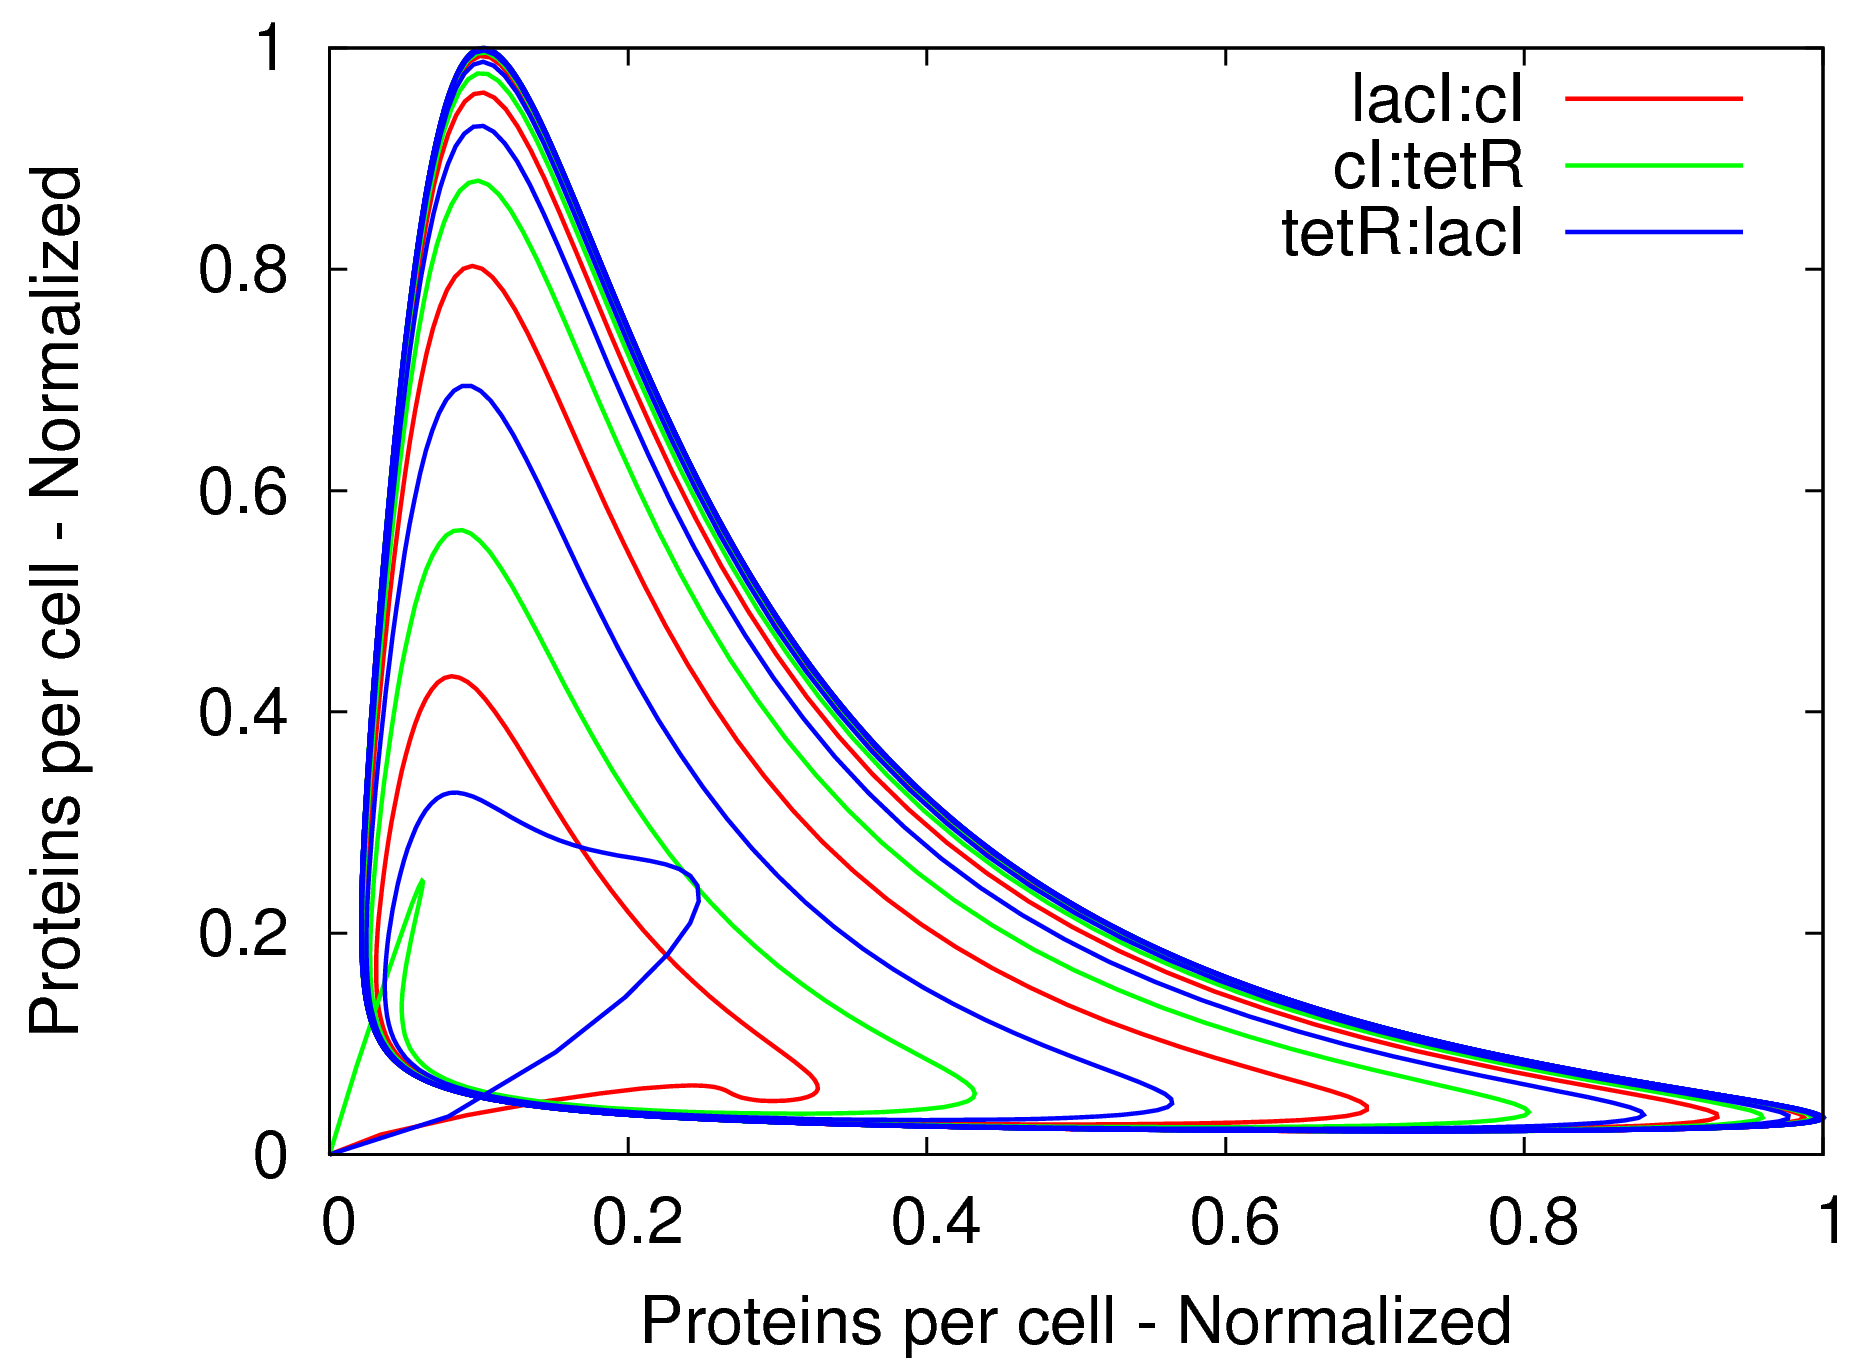
\includegraphics[width=0.7\textwidth]{images/simEx2.png}
\caption{Time-course simulation of the repressilator model, imported from BioModels Database and simulated in COPASI, showing the normalized temporal evolution of repressor proteins lacI, tetR and cI in phase-plane. (taken from \citep{Waltemath:2010})}
\label{fig:simEx2}
\end{figure}
%

%%% Local Variables: 
%%% mode: latex
%%% TeX-master: "../sed-ml-L1V1"
%%% End: 
